\section{The Design of an Intelligent Chatbot with Natural Language Processing Capabilities to Support Learners \cite{wong2022}}
\label{sec:wong2022}

Na transição do ensino secundário para o ensino superior, é comum que os estudantes acabem estranhando a mudança de ambiente \apud{wong2022}{carayannopoulos2018}. Com essa mudança, mesmo alunos que não sejam introvertidos podem não se sentir confortáveis o bastante para tirar dúvidas ou participar das aulas, ocasionando em dificuldades de engajamento na sala de aula. E isso pode causar efeitos negativos no desempenho acadêmico e no desenvolvimento interpessoal dos alunos. 

Apesar de idealmente ser interessante a possibilidade de os docentes darem uma atenção individual para cada aluno, isso é impraticável devido à limitação de tempo dos professores dentro e fora do período das aulas, e ao cansaço que pode acontecer após longos períodos de conversa \apud{wong2022}{clarizia2018}. Com base nessa problemática, o autor avaliou o uso de Chatbots para melhorar a comunicação entre professor e aluno no âmbito acadêmico. Além disso, também foi revisado o uso de tecnologias relacionadas com um propósito similar na educação, como Student Response System (SRS), Learning Management System (LMS) e aplicações Mobile.

% Mover para Fundamentação Teórica os próximos 3 paragráfos
Um Student Response System (SRS) é uma ferramenta eficiente para obter respostas dos alunos em sala de aula. Por meio desse tipo de sistema, é possível para o professor apresentar perguntas para os alunos responderem em seus celulares. Após isso, é possível obter estatísticas das respostas submetidas pelos alunos e discutir elas em classe. Esse uso implica que é necessário que todos ou a maioria dos estudantes submetam suas respostas para dar prosseguimento na aula, o que limita o escopo das questões trabalhadas, visto que a maioria dos professores conseguem trabalhar apenas de três a seis questões por aula \apud{wong2022}{van2017}. Uma outra limitação, é que é possível incluir dicas no enunciado das questões. Entretanto, nem todos os alunos precisam dessas dicas e não há forma de diferenciar quais alunos conseguiram responder corretamente sem fazer uso delas \apud{wong2022}{suleman2016}. Um exemplo popular desse tipo de sistema é o Kahoot.

O Learning Management System (LMS) é um tipo de sistema voltado para a criação de quizzes online. Para \apud{wong2022}{coleman2017}, é comum que os professores passem muito tempo preparando questões nesses sistemas para cobrir diferentes partes do conteúdo. Além disso, esses sistemas costumam não permitir que os estudantes navegam livremente pelo conteúdo em diferentes partes do curso, fazendo a dinâmica do quiz ser mecânica e não atrativa para muitos estudantes. Além do mais, a maioria deles também não conseguem prover um \textit{feedback} personalizado para os alunos com base em suas performances. E como resultado, muitos alunos podem adotar uma abordagem de aprendizado rasa, focando apenas em passar pelo curso realizando o menor esforço possível \apud{wong2022}{biggs2001}. Exemplos conhecidos desse tipo de sistema são o Blackboard e o Moodle.

Muitos sistemas LMS como o Moodle também possuem uma versão Mobile. Entretanto, muitos estudantes acabam hesitando em baixá-las visto que já possuem muitos aplicativos instalados em seu celular \apud{wong2022}{carayannopoulos2018}. Relacionado a isso, também existem preocupações voltadas a segurança, por conta da possibilidade de adquirir um aplicativo malicioso ao baixar esses sistemas.

%Chatbots podem ser definidos como programas de computadores feitos para simular a conversação humana na forma de voz ou texto, ou até mesmo ambos \apud{wong2022}{wales2008}. O primeiro chatbot foi criado em 1966 por Joseph Weizenbaum, e desde então, eles são usados no ensino de áreas como línguas estrangeiras, psicologia e até mesmo como técnicas de entrevista \apud{wong2022}{wales2008,fryer2006,tseng2018}. A maioria da pesquisa em chatbots como uma ferramenta de aprendizado é focada na simulação da capacidade de conversação humana, e estando ela limitada apenas a algumas disciplinas acadêmicas. Assim, dado os avanços e a popularidade que os chatbots vêm ganhando nos últimos anos, surge a necessidade de analisar o potencial deles como uma ferramenta de ensino numa variedade maior de disciplinas.

Para fins do estudo, foi desenvolvido pelo autor um protótipo de chatbot (Figura \ref{fig:chatbot-wong}) usando uma ferramenta de programação visual. Depois disso, ele foi aplicado em uma turma de 27 alunos do último ano de graduação de um curso de ensino superior de programação, como preparação para um quiz online que é parte do exame de certificação da Amazon. Vale ressaltar que tanto o chatbot quanto o quiz fizeram as mesmas dez perguntas, com um acréscimo para o protótipo, que fornecia um feedback textual e com imagens durante a conversação, além de encorajar os usuários quando eles completavam 40\% e 80\% das perguntas. Depois de os estudantes usarem o chatbot, eles fizeram o quiz online da Amazon. Por fim, uma questionário foi aplicado para os participantes.

\begin{figure}[ht] 
   	\captionsetup{width=16cm}
	\Caption{\label{fig:chatbot-wong} Exemplo de conversa do protótipo de chatbot}
	\UFCfig{}{
        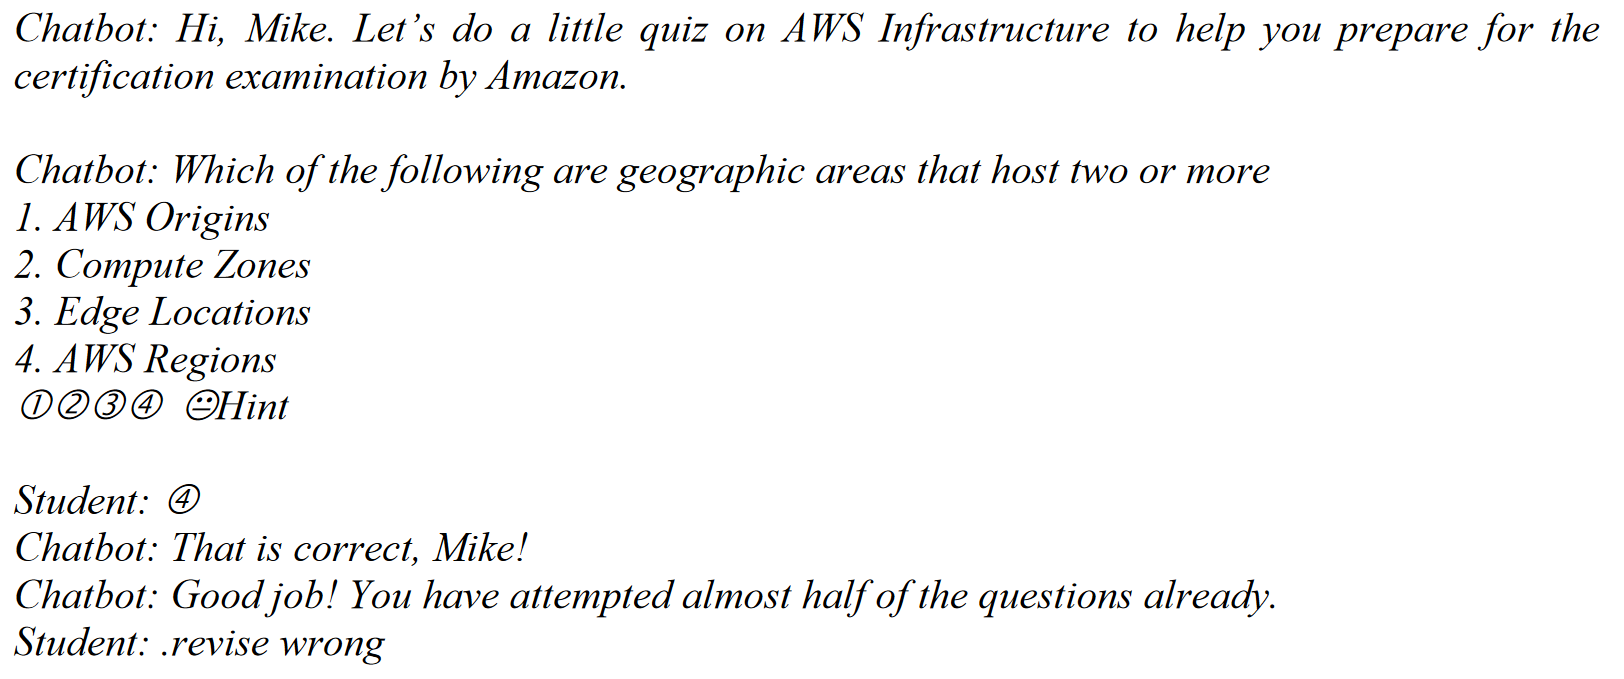
\includegraphics[width=16cm]{figuras/chatbot-wong.png}
    }{
		\Fonte{\citeonline{wong2022}.}
	}
\end{figure}

O questionário mostrou que a maioria dos alunos (de 70\% a 85\%) responderam positivamente para as afirmativas que colocavam o chatbot melhor que o quiz online em vários aspectos. Entretanto, um pouco mais da metade dos alunos (58\%) indicou que eles levaram mais tempo para completar o chatbot que o quiz online. Assim, os beneficiados com esse estudo são professores e alunos, visto que os alunos conseguem obter assistência imediata sobre o conteúdo acadêmico ao acessar o chatbot, e os professores conseguem obter um \textit{feedback} atualizado de como anda o aprendizado dos seus discentes por meio dos resultados coletados pelo chatbot.